\clearpage\section{Chapter 7: Graphics}

Unicon provides a rich high level interface to 2D and 3D raster
graphics, text fonts, colors, and mouse input facilities provided by an
underlying system, such as the X Window System.
Unicon{\textquotesingle}s graphics are portable across multiple
platforms. The most important characteristics of the graphics
facilities are:

\begin{itemize}
\item Simplicity, ease of learning
\item Windows are integrated with Unicon{\textquotesingle}s existing I/O
functions
\item Straightforward input event model
\end{itemize}
This chapter presents an overview of the 2D graphics facilities found in
Unicon and Icon, plus a complete description of the 3D graphics
programming interface in Unicon. Some of the description of 2D graphics
comes from University of Arizona CS TR93-9. The material on 3D graphics
comes from Unicon TR 9, whose primary author is Naomi Martinez. The
definitive reference and programmer{\textquotesingle}s guide for the 2D
graphics facilities is {\textquotedbl}Graphics Programming in
Icon{\textquotedbl} by Griswold, Jeffery, and Townsend, and this book
is also of value for writing 3D programs. Electronic reference manuals
for the graphics facilities also come with the software distributions.

Because different platforms have radically different capabilities, there
is a trade-off between simplicity, portability, and full access to the
underlying machine. Unicon aims for simplicity and ease of programming
rather than full low-level access.

\subsection{The 2D Graphics Interface}

Unicon{\textquotesingle}s 2D facilities provide access to graphics
displays without enforcing a particular user interface look-and-feel.
Events other than keystrokes and mouse events are handled automatically
by the runtime system. Chapter 17 describes the standard class library
and user interface builder for Unicon applications.

Graphic interfaces are \index{event driven}\textit{event driven}; an
event-reading loop is the control mechanism driving the application.
\ For example, if an application must be ready to redraw the contents
of its window at all times, it may not compute for long periods without
checking for window events. The event-driven paradigm is used in the
underlying implementation, but it is optional at the Unicon application
level. \ Since Unicon windows handle many events automatically and
{\textquotedbl}take care of themselves{\textquotedbl}, applications
follow the event-driven paradigm only when it is needed and
appropriate. Unicon{\textquotesingle}s facilities with their extensive
use of default values make simple graphics applications extremely easy
to program, while providing flexibility where it is needed in more
sophisticated applications.

\subsubsection{Window Basics}

Windows are a special file opened with mode
\textsf{{\textquotedbl}g{\textquotedbl},} appearing on-screen as a
rectangular space for text and/or graphics. One can use windows with
the usual file functions, much as one uses a text terminal. A simple
Unicon graphics program might look like this:

\iconcode{
\ \ \ procedure main()\\
 \ \ \ \ \ w := open({\textquotedbl}hello{\textquotedbl},
{\textquotedbl}g{\textquotedbl})\\
 \ \ \ \ \ write(w, {\textquotedbl}hello, world{\textquotedbl})\\
 \ \ \ \ \ \# do processing ... use w as if it were a terminal\\
 \ \ \ \ \ close(w)\\
 \ \ end
}

Windows are open for both reading and writing, and support the usual
file operations with the exceptions of \textsf{seek()} and
\textsf{where()}. \ Unlike regular files, the \textsf{type()} of a
window is {\textquotedbl}window{\textquotedbl}. Like other files,
windows close automatically when the program terminates, so the call to
\textsf{close()} in the above example is optional.

Bit-mapped, or raster, graphics constitute a second programming model
for windows. There are no programming
{\textquotedbl}modes{\textquotedbl} and code that uses graphics may be
freely intermixed with code that performs text operations. \ There are
many graphics functions and library procedures, detailed in Appendices
A and B.

\paragraph{\&window: The Default Window Argument}

The keyword \textsf{\&window} is a default window for graphics I/O.
\ \textsf{\&window} starts out with a null value and is assigned using
the assignment operator. Only window values (and \textsf{\&null}) may
be assigned to \textsf{\&window}. \ \textsf{\&window} is as a default
argument to most graphics functions and is used implicitly by various
operations. If a program uses \textsf{\&window}, the argument can be
omitted from calls to functions such as \textsf{EraseArea()} and
\textsf{WAttrib()}. \ The window argument is required for calls to file
functions such as \textsf{write()} and \textsf{writes()} since these
functions default to \textsf{\&output}, not \textsf{\&window}. \ The
default window shortens the code for graphics-oriented programs and
makes it faster.

\paragraph{2D Graphics Coordinates}

The 2D graphics functions use an integer coordinate system based on
pixels \ (picture elements). \ Like the text coordinate system, 2D
graphics coordinates start in the upper-left corner of the screen.
\ From that corner the positive x direction lies to the right and the
positive y direction moves down. \ Unlike text coordinates, the
graphics coordinate axes are zero-based, which is to say that the very
top leftmost pixel is (0,0) by default.

Angles are real numbers given in radians, clockwise starting with the 3
o{\textquotesingle}clock position. \ Many functions operate on
rectangular regions specified by x, y, width, and height components.
\ Width and height values may be negative to extend the rectangle to
the left or up from x and y. Screen output may be limited to a
rectangular region in the window called the clipping region. The
clipping region is set or unset using the function \textsf{Clip()}.

\paragraph{Window Attributes}
A window{\textquotesingle}s state consists of many \textit{attributes}
with associated values. \ Some values are defined by the system, while
others are under program control. \ In the absence of program-supplied
values, attributes are assigned default values. When opening a window,
\textsf{open()} takes any number of string arguments after the file
name and mode arguments. These arguments specify initial values of
attributes when the window is created. \ For example, to say hello in
italics on a blue background one may write:

\iconcode{
\ \ \ procedure main()\\
 \ \ \ \ \ w := open({\textquotedbl}hello{\textquotedbl},
{\textquotedbl}g{\textquotedbl},
{\textquotedbl}font=sans,italics{\textquotedbl},
{\textquotedbl}bg=blue{\textquotedbl})\\
 \ \ \ \ \ write(w, {\textquotedbl}hello, world{\textquotedbl})\\
 \ \ \ \ \ \# processing ...\\
 \ \ end}

After a window is created, its attributes are inspected and set using
the function \textsf{WAttrib(w,s1,s2,...)}. Arguments to
\textsf{WAttrib()} that include an equals sign are assignments that set
the given value if possible; \textsf{WAttrib()} fails otherwise.
\ \textsf{open()} only contains such attribute assignments. \ Some
attributes can only be read by \textsf{WAttrib()} and not set.

String arguments to \textsf{WAttrib()} that have an attribute name but
no value are queries which return the attribute value.
\textsf{WAttrib()} generates a string result for each argument; a query
on a single argument produces just the value of that attribute; for
multiple arguments and in the case of assignment, the result is the
\textsf{\textit{attr}}\textsf{=}\textsf{\textit{val}} form attribute
assignments take. \ Attributes are also frequently set implicitly by
the user{\textquotesingle}s manipulation of the window; for instance,
cursor or mouse location or window size.

The following attributes are maintained on a per-window basis. \ All
attribute values are string encodings. \ Usage refers to whether the
attribute may be read, written or both. RWO and WO attributes can be
assigned only when the window is \ opened.

\bigskip

{\centering\sffamily\bfseries
Table 7-1

Canvas Attributes
}

\begin{center}
\tablehead{\hline
\centering \bfseries\itshape Name &
\centering \bfseries\itshape Type / Example &
\centering \bfseries\itshape Description &
\centering\arraybslash \bfseries\itshape Usage\\\hline}
\begin{supertabular}{|m{0.9622598in}|m{2.0323598in}|m{2.1712599in}|m{0.44835988in}|}
size &
pixel pair &
Size of window &
RW\\\hline
pos &
pixel pair &
Position of window on screen &
RW\\\hline
canvas &
normal, hidden &
Canvas state &
RW\\\hline
windowlabel &
string &
Window label (title) &
RW\\\hline
inputmask &
string &
select categories of input events &
RW\\\hline
pointer &
arrow, clock &
Pointer (mouse) shape  &
RW\\\hline
pointerx, pointery &
pixel &
Pointer (mouse) location  &
RW\\\hline
display &
device /
{\textquotedbl}hobbes.cs.esu.edu:0{\textquotedbl}
&
(X11) device window resides on &
RWO\\\hline
depth &
\# of bits &
Display depth &
R\\\hline
displaywidth, displayheight &
pixel &
Display size &
R\\\hline
image &
string &
Initial window contents &
WO\\\hline
\end{supertabular}
\end{center}
Although all attribute values are encoded as strings, they represent
very different window system features. The attribute pointer refers to
mouse pointer shapes that may be changed by the application during
different operations. The attribute \textsf{pos} refers to the position
of the upper-left corner of the window on the screen. \ Screen position
is specified by a string containing an x and a y coordinate separated
by a comma, e.g. \textsf{{\textquotedbl}pos=200,200{\textquotedbl}}.

\subsubsection{Graphics Contexts}

Some attributes are associated with the window itself, while others are
associated with the \textit{graphics context}, the set of resources
used by operations that write to windows. \ This distinction is not
necessary in simple applications but is useful in more sophisticated
applications that use multiple windows or draw many kinds of things in
windows. \ A graphics context consists of the colors, patterns, line
styles, and text fonts and sizes.

Although they are called graphics contexts, text operations use these
attributes too: Text is written using the foreground and background
colors and the font defined in the graphics context. \ Table 7-2 lists
the attributes associated with a graphics context.

\pagebreak

{\centering\sffamily\bfseries
Table 7-2
\par}

{\centering\sffamily\bfseries
Context Attributes
\par}

\begin{center}
\tablehead{\hline
\centering \bfseries\itshape Name &
\centering \bfseries\itshape Type / Example &
\centering \bfseries\itshape Description : Default &
\centering\arraybslash \bfseries\itshape Usage\\\hline}
\begin{supertabular}{|m{1.0163599in}|m{1.6261599in}|m{2.5233598in}|m{0.44835988in}|}
fg &
color \ / {\textquotedbl}red{\textquotedbl} &
Foreground color : black &
RW\\\hline
bg &
color \ / {\textquotedbl}0,0,0{\textquotedbl} &
Background color : white &
RW\\\hline
font &
font name &
Text font : fixed &
RW\\\hline
fheight, fwidth &
integer &
Text font max char height and width &
R\\\hline
leading &
integer &
Vertical \# pixels between text lines &
RW\\\hline
ascent, descent &
integer &
Font height above/below baseline &
R\\\hline
drawop &
logical op / reverse  &
Drawing operation: copy &
RW\\\hline
fillstyle &
stippled, opaquestippled &
Graphic fill style : solid &
RW\\\hline
pattern &
{\textquotedbl}4,\#5A5A{\textquotedbl} &
Fill pattern &
RW\\\hline
linestyle &
onoff, doubledash &
Drawing line style : solid  &
RW\\\hline
linewidth &
integer &
Drawing line width &
RW\\\hline
clipx, clipy, clipw, cliph &
integer &
Clip rectangle position and extent: 0 &
RW\\\hline
dx, dy &
integer &
Output coordinate translation : 0 &
R\\\hline
image &
string / {\textquotedbl}flag.xpm{\textquotedbl} &
Initial window contents &
WO\\\hline
\end{supertabular}
\end{center}
\paragraph{Binding Windows and Graphics Contexts Together}
Graphics contexts can be shared among windows, and multiple graphics
contexts can be used on the same window. \ An Unicon window value is a
\textit{binding} of a canvas (an area that may be drawn upon) and a
graphics context. A call
\textsf{open(s,{\textquotedbl}g{\textquotedbl})} creates both a canvas,
and a context, and binds them together, producing the binding as its
return value.

\textsf{Clone(w)} creates a binding with the same canvas and attribute
values as \textsf{w}, having a new graphics context that is manipulated
independently from \textsf{w}. \textsf{Clone()} also accepts any number
of string attributes to apply to the new window value, as in
\textsf{open()} and \textsf{WAttrib()}.

After calling \textsf{Clone()}, two or more Unicon window values can
write to the same canvas. \ The cursor location is stored in the
canvas, not the graphics context. Writing to the windows produces
concatenated (rather than overlapping) output. \ Closing one of those
window values removes the canvas from the screen but does not destroy
its contents; the remaining binding references an invisible pixmap.
\ The canvas is destroyed after the last binding associated with it
closes. Use of \textsf{Clone()} can significantly enhance performance
for applications that otherwise require frequent graphics context
manipulations.

\paragraph{Subwindows}
The function Clone() can also be used to create explicit subwindows,
which are canvases that physically reside within other windows.
\ \textsf{Clone(w, {\textquotedblleft}g{\textquotedblright}, ...)}
opens a 2D subwindow within \textsf{w}, and \textsf{Clone(w,
{\textquotedblleft}gl{\textquotedblright}, ...)} opens a 3D subwindow
within \textsf{w}. \ Applications generally supply position and size
attributes when the call \textsf{Clone()} in this way. \ Input events
to a subwindow are not seen on the enclosing parent window and vice
versa; both windows must be polled or supplied to \textsf{WActive()} or
\textsf{select()} in order to handle input.

\paragraph{Coordinate Translation}
In 2D, context attributes \textsf{dx} and \textsf{dy} perform output
coordinate translation. \textsf{dx} and \textsf{dy} take integer values
and default to zero. \ These integers are added into the coordinates of
all output operations that use the context; input coordinates in
\textsf{\&x} and \textsf{\&y} are not translated.

\subsubsection{Events}

User input such as keystrokes and mouse clicks are called
\textit{events}. Many events are handled by Unicon without intervention
of the programmer, including window redrawing and resizing, etc.
\ Other events are put on a queue in the order they occur, for
processing by the Unicon program. When reading from a window using file
input functions such as \textsf{reads(w, 1)}, only keyboard events are
produced; mouse and other events are dropped.

The primary input function for windows is \textsf{Event(w),} which
produces the next event for window \textsf{w} and removes it from the
queue. If the event queue is empty, \textsf{Event()} waits for an
event. Keyboard events are returned as strings, while mouse events are
returned as integers. \ Special keys, such as function and arrow keys,
are also returned as integers, described below. \textsf{Event()} also
removes the next two elements and assigns the keywords \textsf{\&x} and
\textsf{\&y} the pixel coordinates of the mouse at the time of the
event. The values of \textsf{\&x}, \textsf{\&y} remain available until
a subsequent call to \textsf{Event()} again assigns to them.
\textsf{Event()} sets the keyword \textsf{\&interval} to the number of
milliseconds that have elapsed since the last event (or to zero for the
first event). \ Keywords \textsf{\&control}, \textsf{\&shift}, and
\textsf{\&meta} are set by \textsf{Event()} to return the null value if
those modifier keys were pressed at the time of the event; otherwise
they fail. \ For resize events, \textsf{\&interval} is set to zero and
modifier keywords fail. Keywords associated with event processing on
windows are summarized in Table 7-3:

{\centering\sffamily\bfseries
Table 7-3

Window Input Event Keywords
}

\begin{center}
\tablehead{\hline
\centering \bfseries\itshape Keyword &
\centering\arraybslash \bfseries\itshape Description\\\hline}
\begin{supertabular}{|m{0.91775984in}|m{2.3525598in}|}
\sffamily \&x &
Mouse location, horizontal\\\hline
\sffamily \&y &
Mouse location, vertical\\\hline
\sffamily \&row &
Mouse location, text row\\\hline
\sffamily \&col &
Mouse location, text column\\\hline
\sffamily \&interval &
Time since last event, milliseconds\\\hline
\sffamily \&control &
Succeeds of Control key pressed\\\hline
\sffamily \&shift &
Succceds if Shift key pressed\\\hline
\sffamily \&meta &
Succeeds if Alt (meta) key pressed\\\hline
\end{supertabular}
\end{center}
\paragraph{Keyboard Events}
The regular keys that Unicon returns as one-letter strings correspond
approximately to the lower 128 characters of the ASCII character set.
These characters include the control keys, the escape key, and the
delete key. Modern keyboards have many additional keys, such as
function keys, arrow keys, {\textquotedbl}page down{\textquotedbl},
etc. \ Unicon produces integer events for these special keys. \ A
collection of symbol definitions for special keys is available in the
Icon Program Library include file \textsf{keysyms.icn}. The most common
of these are \textsf{Key\_Down}, \textsf{Key\_Up}, \textsf{Key\_Left},
\textsf{Key\_Right}, \textsf{Key\_Home}, \textsf{Key\_End},
\textsf{Key\_PgUp}, \textsf{Key\_PgDn}, \textsf{Key\_F1...Key\_F12},
and \textsf{Key\_Insert}.

\paragraph{Mouse Events}
Mouse events are returned from \textsf{Event()} as integers indicating
the type of event, the button involved, etc. \ Keywords allow the
programmer to treat mouse events symbolically. The event keywords are:

{\centering\sffamily\bfseries
Table 7-4
\par}

{\centering\sffamily\bfseries
Window Input Event Codes
\par}

\begin{center}
\tablehead{\hline
\centering \bfseries\itshape Keyword &
\centering\arraybslash \bfseries\itshape Event\\\hline}
\begin{supertabular}{|m{0.9247598in}|m{2.3525598in}|}
\sffamily \&lpress &
Mouse press left\\\hline
\sffamily \&mpress &
Mouse press middle\\\hline
\sffamily \&rpress &
Mouse press right\\\hline
\sffamily \&lrelease &
Mouse release left\\\hline
\sffamily \&mrelease &
Mouse release middle\\\hline
\sffamily \&rrelease &
Mouse release right \\\hline
\sffamily \&ldrag &
Mouse drag left \\\hline
\sffamily \&mdrag &
Mouse drag middle \\\hline
\sffamily \&rdrag &
Mouse drag right \\\hline
\sffamily \&resize &
Window was resized \\\hline
\end{supertabular}
\end{center}
The following program uses mouse events to draw a box that follows the
mouse pointer around the screen when a mouse button is pressed. \ The
attribute \textsf{drawop=reverse} allows drawing operations to serve as
their own inverse; see [Griswold98] for more about the \textsf{drawop}
attribute. \ Function \textsf{FillRectangle()} draws a filled rectangle
on the window and is described in the reference section. \ Each time
through the loop the program erases the box at its old location and
redraws it at its new location; the first time through the loop there
is no box to erase so the first call to \textsf{FillRectangle()} is
forced to fail by means of Unicon{\textquotesingle}s
\textsf{{\textbackslash}} operator.

\iconcode{
procedure main()\\
 \ \ \&window := open({\textquotedbl}hello{\textquotedbl},
{\textquotedbl}g{\textquotedbl},
{\textquotedbl}drawop=reverse{\textquotedbl})\\
 \ \ repeat if Event() === (\&ldrag {\textbar} \&mdrag {\textbar}
\&rdrag) then \{\\
 \ \ \ \ \ \# erase box at old position, then draw at new
position\\
 \ \ \ \ \ FillRectangle({\textbackslash}x, {\textbackslash}y, 10,
10)\\
 \ \ \ \ \ FillRectangle(x := \&x, y := \&y, 10, 10)\\
 \ \ \ \ \ \}\\
end}

The Unicon program can inspect the rest of the window{\textquotesingle}s
state using \textsf{WAttrib()}. \ Between the time the mouse event
occurs and the time it is produced by \textsf{Event()}, the mouse may
have moved. \ In order to get the current mouse location, use
\textsf{QueryPointer()} (see below).

When more than one button is depressed as the drag occurs, drag events
are reported on the most recently pressed button. This behavior is
invariant over all combinations of presses and releases of all three
buttons.

Resize events are not mouse events, but they are reported in the same
format. In addition to the event code, \textsf{\&x}, \&y, \&col and
\&row are assigned integers that indicate the window{\textquotesingle}s
new width and height in pixels and in text columns and rows,
respectively. Resize events are produced when the window manager
(usually at the behest of the user) resizes the window; no event is
generated when an Unicon program resizes its window.

\paragraph{Key Release, Mouse Motion, and Window Closure Events}
The canvas attribute inputmask allows programs to request three kinds of
additional input events on windows. These events pose enough
performance or portability obstacles that they are not produced by
default. \ An {\textquotedblleft}m{\textquotedblright} in the inputmask
value requests events for mouse motion events even when no mouse button
is depressed; by default only
{\textquotedblleft}drag{\textquotedblright} events are reported. If the
inputmask contains a {\textquotedblleft}k{\textquotedblright}, events
will be generated when keyboard keys are released. \ An inputmask
attribute containing a {\textquotedblleft}c{\textquotedblright} will
receive an event when a window closure is externally requested or
imposed, as in the case when a titlebar
{\textquotedblleft}x{\textquotedblright} button is pressed.

\paragraph{Event Queue Manipulation}
The event queue is an Unicon list that stores events until the program
processes them. \ When a user presses a key, clicks or drags a mouse,
or resizes a window, three values are placed on the event queue: the
event itself, followed by two integers containing associated event
information.

Pending(w) produces the event queue for window w. If no events are
pending, the list is empty. The list returned by Pending() \ remains
attached to the window, and additional events may be added to it at any
time during program execution. \ Otherwise it is an ordinary list and
can be manipulated using Unicon{\textquotesingle}s list functions and
operators.

When several windows are open, the program may need to wait for activity
on any of the windows and handle it appropriately. This can be
implemented by checking each pending list until a nonempty list is
found, but such a busy-waiting solution is wasteful of CPU time. \ The
function Active() waits for window activity, relinquishing the CPU
until an event is pending on one of the open windows, and then returns
a window with a pending event. A window is said to starve if its
pending events are never serviced. Active() cycles through open windows
on repeated calls in a way that avoids window starvation.

\subsubsection{Colors}

Unicon recognizes a set of string color names based loosely on a color
naming system found in [Berk82]. \ These color names consist of simple
English phrases that specify hue, lightness, and saturation values of
the desired color. \ The syntax of these colors is

[\textit{lightness}] [\textit{saturation}] [\textit{hue}[ish]]
\textit{hue}

where lightness is one of pale, light, medium, dark, or deep; saturation
is one of weak, moderate, strong, or vivid; and where hue is any of
black, gray, grey, white, pink, violet, brown, red, orange, yellow,
green, cyan, blue, purple, or magenta. \ A single space or hyphen
separates each word from its neighbor. \ When two hues are supplied
(and the first hue has no ish suffix), the hue that is specified is
halfway in between the two named hues. \ When a hue with an ish suffix
precedes a hue, the hue that is specified is three-fourths of the way
from the ish hue to the main hue. \ When adding ish to a word ending in
e, the e is dropped (for example, purple becomes purplish); the ish
form of red is reddish. \ Mixing radically different colors such as
yellow and purple does not usually produce the expected results. \ The
default lightness is medium and the default saturation is vivid. \ It
is worth noting that human perception of color varies significantly, as
do the actual colors produced from these names on different monitors.

\paragraph{Color Coordinate Systems and Gamma Correction}
In addition to the standard color names, platform-specific color names
may be supported. Colors may also be specified by strings encoding the
red, green, and blue components of the desired color. Unicon accepts
the hex formats {\textquotedbl}\#rgb{\textquotedbl} in which r, g, and
b are 1 to 4 hex digits each. \ Red, green, and blue may also be given
in decimal format, separated by commas. \ The components are given on a
linear scale from 0 to 65535, although displays typically offer far
less precision and nonlinear colors. For example,
{\textquotedbl}bg=32767,0,0{\textquotedbl} requests a medium red
background; if the display is incapable of such, it approximates it as
closely as possible from the available colors.
{\textquotedbl}fg=0,65000,0{\textquotedbl} requests a vivid green
foreground. If colors appear darker than they should, the window system
is not providing linear colors. Unicon can be told to perform the
correction by means of the gamma attribute; 1.0 is a default (no gamma
correction), and experimenting with values between 2 and 3 usually
provides satisfactory results.

\subsubsection{Fonts}

Fonts are specified by a comma-separated string of up to four fields
supplying the font{\textquotesingle}s family name, followed by optional
size or italic or bold designations in any order. The fonts available
vary widely from system to system. Four font family names available on
all Unicon systems include serif, sans, typewriter, and mono. These
families map onto the system{\textquotesingle}s closest approximation
of Times, Helvetica, Courier, and a monospaced console font. Font sizes
are given in pixel height.

\subsubsection{Images and Palettes}

DrawImage(x, y, s) draws a rectangular area using an image string.
String s has the form
{\textquotedbl}\textit{width},\textit{palette},\textit{data}{\textquotedbl}.
\textit{width} is the width of the rectangle drawn, palette is a code
that defines the colors corresponding to data values, and the rest of
the data supplies pixel values. \ Predefined palettes and palette
functions help to provide this capability. \ Image and palette
functions are described fully in [Griswold98].

\subsubsection{Patterns}

Graphics contexts include a fillstyle attribute that determines the
pixels drawn during draw and fill operations such as rectangles, arcs,
and polygons. \ If the fillstyle is not solid, a selected pattern in
the filled area is drawn in the foreground color; other pixels are
drawn in the background color
({\textquotedbl}fillstyle=textured{\textquotedbl}). \ Patterns are
specified by the function Pattern(w,s), which associates a pattern
denoted by s with w{\textquotesingle}s context. \ String s is either
the name of a standard pattern, or a representation of the bits that
define the pattern. Pattern representations are of the form
{\textquotedbl}width,\#bits{\textquotedbl} where 1 {\textless}= width
{\textless}= 32. The window system may define a limit as low as 8 on
the pattern{\textquotesingle}s width and height.

The height of the pattern is defined by the number of rows in the bits
component of the pattern string. \ Bits consists of a series of
numbers, each supplying one row of the pattern, in hexadecimal format.
Each digit defines four bits and each row is defined by the number of
digits required to supply width bits. \ For example, the call

\iconcode{
\>   Pattern({\textquotedbl}4,\#5A5A{\textquotedbl})}

\noindent defines a 4x4 pattern where each row is defined by one hex digit.

\subsubsection{Pme: a Pixmap Editor}

A simple image editor called Pme, demonstrates event processing
including mouse events. \ Pme displays both a small and a
{\textquotedbl}magnified{\textquotedbl} display of the image being
edited, allows the user to set individual pixels, and allows the user
to save the image; it is well-suited for constructing and hand-editing
small images such as icons and textures for use in larger 2D or 3D
scenes. \ Pme consists of four procedures and employs several graphics
functions. A sample screen image of pme is presented in Figure 7-1. The
{\textquotedblleft}real{\textquotedblright} image is in the upper left
corner; underneath it is a mouse icon which shows what color is drawn
by each of the mouse buttons.



\begin{center}
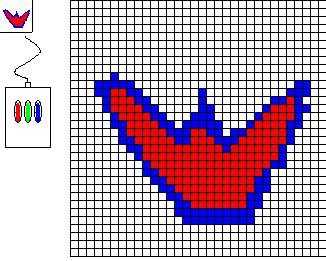
\includegraphics[width=1.7917in,height=1.3575in]{ub-img/ub-img11.jpg}
\end{center}

{\sffamily\bfseries Figure 7-1}
{\sffamily Pme editing a 32x32 image}

\bigskip

Pme starts by declaring and initializing several variables.

\bigskip

\iconcode{
link dialog \\
link file\_dlg \\
global lmargin, colors, colorbinds \\
procedure main(argv) \\
\>   local i := 1, j, s, e, x, y, width := 32, height := 32
}

The image width and height can be specified on the command line with a
{}-size option, for example, \ pme -size 16,64.

\iconcode{
\>   if argv[1]=={\textquotedbl}-size{\textquotedbl} then \{ \\
\>   \ \ \ i +:= 1 \\
\>   \ \ \ argv[2] ? \{ \\
\>   \ \ \ \ \ \ width := integer(tab(many(\&digits))) {\textbar}
stop({\textquotedbl}bad -size{\textquotedbl}) \\
\>   \ \ \ \ \ \ ={\textquotedbl},{\textquotedbl} {\textbar}
stop({\textquotedbl}bad -size{\textquotedbl}) \\
\>   \ \ \ \ \ \ height := integer(tab(0)) {\textbar}
stop({\textquotedbl}bad -size{\textquotedbl}) \\
\>   \ \ \ \ \ \ i +:= 1 \\
\>   \ \ \ \ \ \ \} \\
\>   \ \ \ \}
}

Following the size arguments, Pme checks for a filename specifying the
bitmap to edit. \ If one is found, it is read into the regular scale
image, and then the magnified scale image is constructed by reading
each pixel using the function \textsf{Pixel()}, and filling an 8x8
rectangle with the corresponding color.

\iconcode{
\>   \ \ \ i := j := 0 \\
\>   \ \ \ every p := Pixel(0, 0, width, height) do \{ \\
\>   \ \ \ \ \ \ Fg(p) \\
\>   \ \ \ \ \ \ FillRectangle(j * 8 + lmargin + 5, i * 8, 8, 8) \\
\>   \ \ \ \ \ \ j +:= 1 \\
\>   \ \ \ \ \ \ if j = width then \{ i +:= 1; j := 0 \} \\
\>   \ \ \ \ \ \ \}
}

After the images are loaded with their initial contents, if any, a grid
is drawn on the magnified image to delineate each individual
pixel{\textquotesingle}s boundary. \ The user{\textquotesingle}s mouse
actions within these boxes change the colors of corresponding pixels in
the image. An list of three bindings to the window, each with an
independently-set foreground color, is used to represent the color
settings of the mouse buttons.

\iconcode{
\>   colors :=
[Clone({\textquotedbl}fg=red{\textquotedbl}),Clone({\textquotedbl}fg=green{\textquotedbl}),Clone({\textquotedbl}fg=blue{\textquotedbl})]
}

The main event processing loop of pme is simple: Each event is fetched
with a call to \textsf{Event()} and immediately passed into a case
expression. \ The keystroke \textsf{{\textquotedbl}q{\textquotedbl}}
exits the program; the keystroke
\textsf{{\textquotedbl}s{\textquotedbl}} saves the bitmap in a file by
calling \textsf{WriteImage()}, asking for a file name if one has not
yet been supplied.

\iconcode{
\>   \ \ \ case e := Event() of \{ \\
\>   \ \ \ {\textquotedbl}q{\textquotedbl}{\textbar}{\textquotedbl}{\textbackslash}e{\textquotedbl}:
return \\
\>   \ \ \ {\textquotedbl}s{\textquotedbl}{\textbar}{\textquotedbl}S{\textquotedbl}:
\{ \\
\>   \ \ \ \ \ \ if /s {\textbar} (e=={\textquotedbl}S{\textquotedbl})
then s := getfilename() \\
\>   \ \ \ \ \ \ write({\textquotedbl}saving image {\textquotedbl}, s,
{\textquotedbl} size {\textquotedbl},
width,{\textquotedbl},{\textquotedbl}, height) \\
\>   \ \ \ \ \ \ WriteImage( s, 0, 0, width, height) \\
\>   \ \ \ \ \ \ \}
}

Mouse events in one of the images result in the drawing of a single
pixel in both the magnified and regular scale bitmaps using one of the
colors depicted on the mouse icon. 

\iconcode{
\>   \ \ \ \&lpress {\textbar} \&ldrag {\textbar} \&mpress {\textbar}
\&mdrag {\textbar} \&rpress {\textbar} \&rdrag : \{ \\
\>   \ \ \ \ \ \ x := (\&x - lmargin - 5) / 8 \\
\>   \ \ \ \ \ \ y := \&y / 8 \\
\>   \ \ \ \ \ \ if (y {\textless} 0) {\textbar} (y {\textgreater}
height-1) {\textbar} (x {\textgreater} width) then next \\
\>   \ \ \ \ \ \ if x {\textgreater}= 0 then dot(x, y, (-e - 1) \% 3)
}

To change the color drawn by a mouse button, you click on it.

\iconcode{
\>   \ \ \ \ \ \ else \{ \# x {\textless} logical 0. User clicked in
mouse area \\
\>   \ \ \ \ \ \ \ \ \ if \&x {\textless} 21 then getacolor(1,
{\textquotedbl}left{\textquotedbl}) \\
\>   \ \ \ \ \ \ \ \ \ else if \&x {\textless} 31 then getacolor(2,
{\textquotedbl}middle{\textquotedbl}) \\
\>   \ \ \ \ \ \ \ \ \ else getacolor(3,
{\textquotedbl}right{\textquotedbl}) \\
\>   \ \ \ \ \ \ \ \ \ until Event() === (\&mrelease {\textbar}
\&lrelease{\textbar} \&rrelease) \\
\>   \ \ \ \ \ \ \ \ \ \} \\
\>   \ \ \ \ \ \ \}
}

Pixel drawing is handled identically by procedure dot(), whose third
argument specifies which button, and therefore which color to draw.
\ The dot is drawn using FillRectangle() in the magnified window; in
the regular scale window DrawPoint() suffices.

\iconcode{
procedure dot(x, y, c) \\
\>   if (x{\textbar}y) {\textless} 0 then fail \\
\>   FillRectangle(colors[c+1], x*8 + lmargin + 5, y*8, 8, 8) \\
\>   DrawPoint(colors[c+1], x, y) \\
\>   DrawRectangle(x*8 + lmargin + 5, y*8, 8, 8) \\
end
}

Pme illustrates several aspects of the Unicon graphics facilities. Note
the event-handling: a single case expression that handles various
keystrokes and mouse events as different cases makes the control
structure simpler than in many languages{\textquotesingle} GUI event
processing.

\bigskip

{\sffamily\bfseries Listing 7-1}
{\sffamily\bfseries Pme: a Unicon bitmap editor}

\iconcode{
link dialog \\
link file\_dlg \\
global lmargin, colors \\
procedure main(argv) \\
\>   local i := 1, j, s, e, x, y, width := 32, height := 32 \\
\>   if argv[1]=={\textquotedbl}-size{\textquotedbl} then \{ \\
\>   \ \ \ i +:= 1 \\
\>   \ \ \ argv[2] ? \{ \\
\>   \ \ \ \ \ \ width := integer(tab(many(\&digits))) {\textbar}
stop({\textquotedbl}bad -size{\textquotedbl}) \\
\>   \ \ \ \ \ \ ={\textquotedbl},{\textquotedbl} {\textbar}
stop({\textquotedbl}bad -size{\textquotedbl}) \\
\>   \ \ \ \ \ \ height := integer(tab(0)) {\textbar}
stop({\textquotedbl}bad -size{\textquotedbl}) \\
\>   \ \ \ \ \ \ i +:= 1 \\
\>   \ \ \ \ \ \ \} \\
\>   \ \ \ \} \\
\>   lmargin := max(width, 65) \\
\>   if s := argv[i] then \{ \\
\>   \ \ \ \&window := open({\textquotedbl}pme{\textquotedbl},
{\textquotedbl}g{\textquotedbl},
{\textquotedbl}image={\textquotedbl}{\textbar}{\textbar}s) {\textbar}
stop({\textquotedbl}cannot open window{\textquotedbl}) \\
\>   \ \ \ width \ {\textless}:=
WAttrib({\textquotedbl}width{\textquotedbl}) \\
\>   \ \ \ height {\textless}:=
WAttrib({\textquotedbl}height{\textquotedbl}) \\
\>   \ \ \ lmargin := max(width, 65) \\
\>   \ \ \ WAttrib({\textquotedbl}size={\textquotedbl}{\textbar}{\textbar}(width*8+lmargin+5){\textbar}{\textbar}{\textquotedbl},{\textquotedbl}{\textbar}{\textbar}(height*8)) \\
\>   \ \ \ i := j := 0 \\
\>   \ \ \ every p := Pixel(0, 0, width, height) do \{ \\
\>   \ \ \ \ \ \ Fg(p) \\
\>   \ \ \ \ \ \ FillRectangle(j * 8 + lmargin + 5, i * 8, 8, 8) \\
\>   \ \ \ \ \ \ j +:= 1 \\
\>   \ \ \ \ \ \ if j = width then \{ i +:= 1; j := 0 \} \\
\>   \ \ \ \ \ \ \} \\
\>   \ \ \ \} \\
\>   else \{ \\
\>   \ \ \ \&window := open({\textquotedbl}pme{\textquotedbl},
{\textquotedbl}g{\textquotedbl},
{\textquotedblright}size={\textquotedblright} {\textbar}{\textbar}
(lmargin+width*8+5){\textbar}{\textbar}{\textquotedbl},{\textquotedbl}{\textbar}{\textbar}(height*8+5))
{\textbar} \\
 \ \ \ \ \ \ \ \ stop({\textquotedbl}cannot open window{\textquotedbl}) \\
\>   \ \ \ \} \\
\>   colors :=
[Clone({\textquotedbl}fg=red{\textquotedbl}),Clone({\textquotedbl}fg=green{\textquotedbl}),Clone({\textquotedbl}fg=blue{\textquotedbl})] \\
\>   every i := 1 to 3 do \{ \\
\>   \ \ \ DrawArc(4+i*10, height+68, 7, 22) \\
\>   \ \ \ FillArc(colors[i], 5+i*10, height+70, 5, 20) \\
\>   \ \ \ \} \\
\>   DrawRectangle( 5, height+55, 45, 60, 25, height+50, 5, 5) \\
\>   DrawCurve(27, height+50, 27, height+47, 15, height+39, \\
\>   \ \ \ \ \ \ \ \ \ \ 40, height+20, 25, height+5) \\
\>   Fg({\textquotedbl}black{\textquotedbl}) \\
\>   every i := 0 to height-1 do \\
\>   \ \ \ every j := 0 to width-1 do \\
\>   \ \ \ \ \ \ DrawRectangle(j*8+lmargin+5, i*8, 8, 8) \\
\>   DrawLine(0, height, width, height, width, 0) \\
\>   repeat \{ \\
\>   \ \ \ case e := Event() of \{ \\
\>   \ \ \ {\textquotedbl}q{\textquotedbl}{\textbar}{\textquotedbl}{\textbackslash}e{\textquotedbl}:
return \\
\>   \ \ \ {\textquotedbl}s{\textquotedbl}{\textbar}{\textquotedbl}S{\textquotedbl}:
\{ \\
\>   \ \ \ \ \ \ if /s {\textbar} (e=={\textquotedbl}S{\textquotedbl})
then s := getfilename() \\
\>   \ \ \ \ \ \ write({\textquotedbl}saving image {\textquotedbl}, s,
{\textquotedbl} size {\textquotedbl},
width,{\textquotedbl},{\textquotedbl}, height) \\
\>   \ \ \ \ \ \ WriteImage( s, 0, 0, width, height) \\
\>   \ \ \ \ \ \ \} \\
\>   \ \ \ \&lpress {\textbar} \&ldrag {\textbar} \&mpress {\textbar}
\&mdrag {\textbar} \&rpress {\textbar} \&rdrag : \{ \\
\>   \ \ \ \ \ \ x := (\&x - lmargin - 5) / 8 \\
\>   \ \ \ \ \ \ y := \&y / 8 \\
\>   \ \ \ \ \ \ if (y {\textless} 0) {\textbar} (y {\textgreater}
height-1) {\textbar} (x {\textgreater} width) then next \\
\>   \ \ \ \ \ \ if x {\textless} 0 then \{ \\
\>   \ \ \ \ \ \ \ \ \ if \&x {\textless} 21 then getacolor(1,
{\textquotedbl}left{\textquotedbl}) \\
\>   \ \ \ \ \ \ \ \ \ else if \&x {\textless} 31 then getacolor(2,
{\textquotedbl}middle{\textquotedbl}) \\
\>   \ \ \ \ \ \ \ \ \ else getacolor(3,
{\textquotedbl}right{\textquotedbl}) \\
\>   \ \ \ \ \ \ \ \ \ until Event(w) === (\&mrelease {\textbar}
\&lrelease{\textbar} \&rrelease) \\
\>   \ \ \ \ \ \ \ \ \ \} \\
\>   \ \ \ \ \ \ else dot(x, y, (-e-1)\%3) \\
\>   \ \ \ \ \ \ \} \\
\>   \ \ \ \} \\
\>   \} \\
end
\ \\
procedure dot(x, y, c) \\
\>   if (x{\textbar}y) {\textless} 0 then fail \\
\>   FillRectangle(colors[c+1], x*8 + lmargin + 5, y*8, 8, 8) \\
\>   DrawPoint(colors[c+1], x, y) \\
\>   DrawRectangle( x*8 + lmargin + 5, y*8, 8, 8) \\
end
\ \\
procedure getacolor(n, s) \\
\>   if ColorDialog([{\textquotedbl}Set
{\textquotedbl}{\textbar}{\textbar}s{\textbar}{\textbar}{\textquotedbl}
button color{\textquotedbl}], Fg(colors[n])) == \\
\>   \ \ \ \ \ \ {\textquotedbl}Okay{\textquotedbl} then \{ \\
\>   \ \ \ Fg(colors[n], dialog\_value) \\
\>   \ \ \ FillArc(colors[n], 5 + n * 10, height + 70, 5, 20) \\
\>   \} \\
end
\ \\
procedure getfilename() \\
\>   f := FileDialog() \\
\>   f.show\_modal() \\
\>   return f.file.contents \\
end
}

\subsection{The 3D Graphics Interface}

Three-dimensional graphics are provided in Unicon on platforms which
support the industry standard OpenGL libraries. Unicon provides the
basic primitives, transformations, lighting, and texturing \ elements
of 3D computer graphics in a simplified fashion, providing a good basis
to rapidly construct 3D scenes. The Unicon 3D interface consists of
sixteen new functions and six functions that were extended from the 2D
graphics facilities, compared with OpenGL{\textquotesingle}s 250+
functions. While Unicon{\textquotesingle}s 3D interface vastly
simplifies some aspects of 3D programming compared with the OpenGL C
interface, it does not currently provide access to several features of
OpenGL including blending, fog, anti aliasing, display lists,
selection, and feedback.

This section explains in detail how to use Unicon{\textquotesingle}s 3D
facilities, for programmers who already have some idea of how 3D
graphics work. A 3D window is opened using mode
{\textquotedbl}gl{\textquotedbl} and is very similar to a 2D window, so
much of the previous sections of this chapter are needed for 3D
programming. 3D graphics use the 2D windowing functions and attributes
and introduce several new ones.

A primary difference between 2D and 3D is that graphics operations in 2D
windows use (x,y) integer pixel coordinates defined relative to the
upper left corner of the window, while 3D windows use (x,y,z) real
number coordinates in an abstract geometric world in which a mobile
viewer{\textquotesingle}s position, and the direction they are looking,
determine what is visible. Coordinates of 3D objects go through a
series of translations, scalings, and rotations to determine their
final location; these matrix transformations are used to compose
aggregate objects from their parts. In addition to the coordinate
system difference, 3D scenes usually employ a rich lighting model, and
use materials and textures to draw objects more frequently than a solid
foreground color. For this reason, the fg attribute is extended in the
3D realm to denote a foreground \textit{material}, including color as
well as how the object appears in different types of lighting.

\subsubsection{Opening Windows for 3D Graphics}

To open a 3D graphics window, call the built in function open(), passing
in the title of the window to be opened and \ mode
{\textquotedbl}gl{\textquotedbl}.

\iconcode{
\>   W := open({\textquotedbl}win{\textquotedbl},
{\textquotedbl}gl{\textquotedbl})}

As in the 2D facilities, if a window is assigned to the keyword variable
\&window, it is a default window for subsequent 3D function calls. 

\subsubsection{3D Attributes}

Features such as lighting, perspective, texturing, and shading, give a
scene the illusion of being three-dimensional. In order to control such
features, a Unicon programmer makes use of context attributes. By
assigning new values to various attributes the programmer can control
many aspects of the scene. Attributes to control the coordinate system,
field of view, lighting and textures are included in the Unicon 3D
graphics facilities. 

Some of the most basic context attributes concern the coordinate system.
In 3D graphics \ an x-coordinate, a y-coordinate, and a z-coordinate
determine where to place an object. The objects that are visible on the
screen depend on several things, the eye position, the eye direction,
and the orientation of the scene. If these items are not taken into
account, the scene \ desired by the user and the scene drawn may be two
very different things. 

To think about these attributes, imagine a person walking around a 3D
coordinate system. What the person sees becomes the scene viewed on the
screen. The eye position specifies where the person is standing. Things
close to the person appear larger and seem closer than objects further
away. The eye direction specifies where the person is looking. If the
person is looking toward the negative z-axis, only the objects situated
on the negative z-axis are viewed in the scene. Anything on the
positive z-axis is behind the viewer. Finally, the up direction can be
described by what direction is up for the person. 

The eye position is given by the attribute eyepos. By default this is
set to be at the origin or (0, 0, 0). The eye direction is given by the
attribute eyedir. By default this is set to be looking at the negative
z-axis. The up direction can be specified by the attribute eyeup and by
default is (0, 1, 0). The attribute eye allows the user to specify
eyepos, eyedir, and eyeup with a single value. Changing any of these
attributes causes the scene to redraw itself with the new eye
specifications.

\subsubsection{3D Drawing Primitives}

In 2D, a user can draw points, lines, polygons, and circles. Functions
from the 2D facilities that have been extended for 3D include
DrawPoint()\textsf{, }DrawLine()\textsf{, }DrawSegment()\textsf{,
}DrawPolygon()\textsf{, }and\textsf{ }FillPolygon(). The 3D facilities
introduce many new primitives, including cubes, spheres, tori,
cylinders, and disks. These are described in Table 7-5 below.

Many scenes are drawn using a mixture of 2D, 3D and 4D objects. The
context attribute \textsf{dim} allows the program to switch between the
different dimensions when specifying the vertices an objects. A user
can draw 2D, 3D, or 4D objects by assigning \textsf{dim} the values of
2, 3, or 4. For primitives that take x, y, and z coordinates,
specifying only x and y coordinate is not sufficient. For this reason,
\textsf{{\textquotedblleft}dim = 2{\textquotedblright}} disallows the
use of these primitives. These functions are
\textsf{DrawSphere()}\textsf{, }\textsf{DrawTorus()}\textsf{,
}\textsf{DrawCube()}\textsf{, and }\textsf{DrawCylinder()}.\texttt{ }By
default the value of \textsf{dim} is three.

\bigskip

% \clearpage
{\centering\sffamily\bfseries
Table 7-5
\par}

{\centering\sffamily\bfseries
Types of 3D Primitives
\par}

\begin{center}
\tablehead{}
\begin{supertabular}{|m{0.75in}|m{1.1in}|m{2.8in}|m{1.0in}|}
\hline
Primitive &
Function &
Parameters &
Picture\\\hline
Cube &
DrawCube() &
the x, y, and z coordinates of the lower left front corner, and the
length of the sides.  &
\centering\arraybslash 
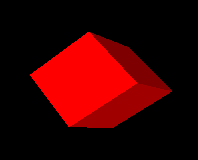
\includegraphics[width=0.9543in,height=0.772in]{ub-img/ub-img12.png}
\\\hline
Cylinder &
DrawCylinder() &
the x, y, and z coordinates of the center, the height, the radius of the
top, the radius of the bottom. If one radius is smaller than the other
a cone is formed. \  &
\centering\arraybslash 
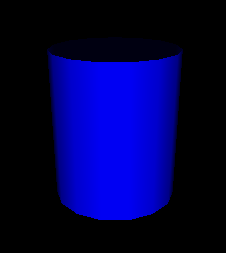
\includegraphics[width=0.7984in,height=0.689in]{ub-img/ub-img13.png} 
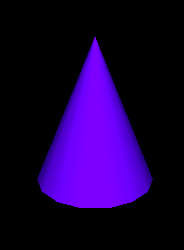
\includegraphics[width=0.7953in,height=0.689in]{ub-img/ub-img14.png}
\\\hline
Disk &
DrawDisk() &
the x, y, and z coordinates of center, the radius of the inner circle,
and the radius of the outer circle. By specifying an additional two
angle values a partial disk is obtained.  &
{\centering 

\includegraphics[width=0.7866in,height=0.689in]{ub-img/ub-img15.png}
\par}

\centering\arraybslash 

\includegraphics[width=0.7866in,height=0.689in]{ub-img/ub-img16.png}
\\\hline
Solid Polygon &
FillPolygon() &
the x, y, and z coordinates of each vertex of the polygon.  &
\centering\arraybslash 

\includegraphics[width=0.9429in,height=0.6217in]{ub-img/ub-img17.png}
\\\hline
Line &
DrawLine() &
the x, y, and z coordinates of each vertex of the line.  &
\centering\arraybslash 
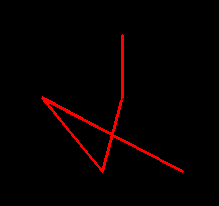
\includegraphics[width=0.9417in,height=0.5957in]{ub-img/ub-img18.png}
\\\hline
Polygon &
DrawPolygon() &
the x, y, and z coordinates of each vertex of the polygon.  &
\centering\arraybslash 
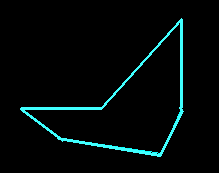
\includegraphics[width=0.9417in,height=0.6043in]{ub-img/ub-img19.png}
\\\hline
Point &
DrawPoint() &
the x, y, and z coordinates of each individual point. &
\centering\arraybslash 
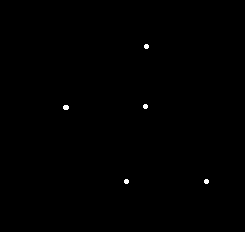
\includegraphics[width=0.9429in,height=0.5957in]{ub-img/ub-img20.png}
\\\hline
Segment &
DrawSegment() &
the x, y, and z coordinates of each vertex of the line segments. &
\centering\arraybslash 
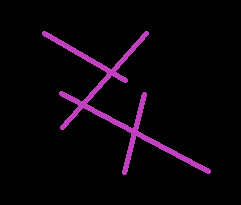
\includegraphics[width=0.9362in,height=0.6425in]{ub-img/ub-img21.png}
\\\hline
Sphere &
DrawSphere() &
the x, y, and z coordinates of center and the radius of the sphere.  &
\centering\arraybslash 
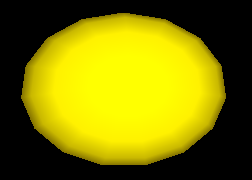
\includegraphics[width=0.9307in,height=0.6543in]{ub-img/ub-img22.png}
\\\hline
Torus &
DrawTorus() &
the x, y, and z coordinates of the center, an inner radius and an outer
radius.  &
\centering\arraybslash 
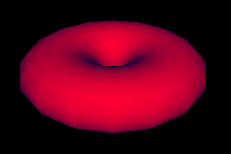
\includegraphics[width=0.9398in,height=0.6272in]{ub-img/ub-img23.png}
\\\hline
\end{supertabular}
\end{center}
\subsubsection[Coordinate Transformations]{Coordinate Transformations}
Matrix multiplications are used to calculate transformations, such as
rotations, translations, and scaling, on objects and the field of view.
Functions to perform several matrix operations in support of coordinate
transformation are available. The main transformation functions are
\textsf{Translate(dx,dy,dz)}, \textsf{Scale(mx,my,mz)}, and
\textsf{Rotate(a,x,y,z)}.

In many 3D graphics applications, transformations are composed as the
pieces of an object are drawn relative to one another. Transformations
are saved and restored as objects are traversed. OpenGL keeps track of
the current matrix with a stack of matrices, where the top of the stack
is the current matrix. The Unicon 3D graphics facilities use
OpenGL{\textquotesingle}s implementation of matrix stacks to implement
transformations. 

Several functions manipulate the matrix stack. The function
\textsf{PushMatrix()} pushes a copy of the current matrix onto the
stack. By doing this the user can compose several different
transformations. The function \textsf{IdentityMatrix()} changes the
current matrix to the identity matrix. To discard the top matrix and to
return to the previous matrix, the function
\textsf{PopMatrix()}\textsf{ }pops the top matrix off the matrix stack.


There are different matrix stacks for the projection and modelview. The
projection matrix stack contains matrices that perform calculations on
the field of view. These calculations are based on the current eye
attributes. If these eye attributes are changed, then previous
manipulations of the projection matrix stack are no longer valid. The
maximum depth of the projection matrix stack is two. Trying to push
more than two matrices onto the projection matrix stack will generate a
runtime error. The modelview matrix stack contains matrices to perform
calculations on objects within the scene. Transformations formed using
the matrix stack only effect the objects that a programmer desires. The
maximum depth of this stack is 32. So, pushing more than 32 matrixes on
the modelview stack will generate an error. Furthermore, only one
matrix stack can be manipulated at any given time. The function
\textsf{MatrixMode()}\textsf{ }switches between the two matrix stacks. 

\subsubsection{Lighting and Materials}

The use of lighting is an important step in making a 3D graphics scene
appear to be 3D. Adding lighting to a scene can be fairly complicated.
A light source can emit different types of light: ambient light,
diffuse light, and specular light. \ Ambient light is light that has
been scattered so much that is difficult to determine the source.
Backlighting in a room is an example of ambient light. Diffuse light
comes from one direction. This type of light mostly defines what color
the object appears to be. Finally, specular light not only comes from
one direction, but also tends to bounce off the objects in the scene.

Applications control lighting using context attributes. For a 3D scene
in Unicon, there are eight lights available. Attributes \textsf{light0}
through \textsf{light7} control the eight lights. Each light is
\textsf{on} or \textsf{off} and has the properties \textsf{diffuse},
\textsf{ambient}, \textsf{specular}, and \textsf{position}. 

A scene not only has several lights, but the objects in scene may have
several material properties. The material properties are ambient,
diffuse, and specular, which are similar to the light properties, plus
emission, and shininess. If an object has an emission property, it
emits light of a specific color. Using combinations of these material
properties one can give an object the illusion of being made of plastic
or metal.

In the 2D facilities, the current foreground color is controlled using
the attribute fg. In 3D, the fg attribute is extended to allow a
semi-colon separated list of material properties with the color that
property should have. The values for each of the lights follow the same
pattern. A programmer can specify colors as in the 2D graphics
facilities, or by providing comma-separated red, green, and blue
intensities as real numbers between \textsf{0.0} and \textsf{1.0}.
\ Examples of lighting and material properties can be found below.

By extending the design of the 2D graphics facilities, the specification
of lights and materials is simplified. The foreground attribute greatly
reduces the number of lines of code needed for a scene. Thanks to this
design along with the extensive use of defaults, a programmer can use
lighting in a 3D graphics application without much effort.

\subsubsection[Textures]{Text\textstyleHeadingivChar{u}res}
Another important area of three-dimension computer graphics is textures.
Adding textures to a scene can give a scene a realistic feel. In order
to implement textures in the Unicon 3D graphics facilities, several
aspects of texturing have to be taken into account. A texture image can
be viewed as a rectangular image that is
{\textquotedbl}glued{\textquotedbl} onto objects in a scene. The
appearances of the textured objects in the scene depend on several key
pieces of information supplied by the programmer. These include the
texture image and what parts of the texture image is mapped to what
parts of an object.

The attribute texmode controls whether a scene uses textures, which are
disabled by default.
\ Wattrib({\textquotedbl}texmode=on{\textquotedbl}) enables textures.
Once textures are enabled and a texture image is given, the texture
will be applied to subsequent objects in the scene. 

Unicon provides several formats to specify a texture image. A texture
can be another Unicon window, an image file, or a string. If the
texture image is a string it is encoded in one of the language standard
formats {\textquotedbl}width,pallet,data{\textquotedbl} or
{\textquotedbl}width,\#data{\textquotedbl} described in the 2D graphics
facilities. In the first case the pallet will determine what colors
appear in the texture image. In the second case, the foreground color
and background color are used. \ The ability to use another Unicon
window as a texture provides great flexibility for texture images,
allowing programs to create texture images dynamically.

Textures must have a height of \ 2\textsuperscript{n} pixels and width
of 2\textsuperscript{m} pixels where n and m are integers. If not, the
texture dimensions are automatically scaled down to the closest power
of 2. Rescaling affects application performance and may cause visual
artifacts, so it may be wise to create textures with appropriate sizes
in the first place. Examples of how to use textures specified in the
different forms are given below.

A programmer can specify a texture either by calling
\textsf{WAttrib({\textquotedbl}texture=...{\textquotedbl})}\textsf{ }or
using \textsf{Texture(t)}. These methods differ in one important way: a
window cannot be used as a texture with \textsf{WAttrib(),} so
\textsf{Texture()} must be called when a window is used as a texture.

A program can specify how a texture is applied to particular object.
This is done by specifying texture coordinates and vertices. Texture
coordinates are x and y coordinates of the texture image. The texture
coordinate (0.0, 0.0) corresponds to the lower left corner of the
texture image. Texture coordinates are mapped to the vertices of an
object in the scene. Together, the texture coordinates and the vertices
determine what the scene looks like after textures have been applied.
Since texture coordinates are complex, defaults are provided. Assigning
attribute \textsf{texcoord} the value \textsf{auto} causes system
default texture coordinates to be used. The defaults are dependent on
the type of primitive.

Non-default texture coordinates are given in several ways, such as \linebreak
\textsf{WAttrib({\textquotedbl}texcoord=}\textsf{\textit{s{\textquotedbl}}}\textsf{)}
where \textsf{\textit{s}} is a comma separated string of real number
values between \textsf{0.0} and \textsf{1.0}. \ Each pair of values is
taken as one texture coordinate; there must be an even number of
decimal values or the assignment of texture coordinates will fail. One
can assign texture coordinates by calling \textsf{Texcoord(x1,y1,...)}
where each \textsf{x} and \textsf{y} are real number values between
\textsf{0.0} and \textsf{1.0}. Finally one can use \textsf{Texcoord(L)}
where \textsf{L} is a list of real number texture coordinates. The
texture coordinates specified by the programmer are used differently
depending on the type of primitive to be drawn. If the primitive is a
point, line, line segment, polygon, or filled polygon, then a texture
coordinate given is assigned to each vertex. If there are more texture
coordinates than vertices, unused texture coordinates are ignored. If
there are more vertices than texture coordinates the application of a
texture will fail. \ In order to use non default texture coordinates
with cubes, tori, spheres, disks, and cylinders a programmer should
approximate the desired mapping with filled polygons. These
specifications are given in Table 7-6.

% \clearpage

{\centering\sffamily\bfseries
Table 7-6
\par}

{\centering\sffamily\bfseries
Texture coordinates and primitives
\par}

\begin{center}
\tablehead{}
\begin{supertabular}{|m{0.7122598in}|m{3.22956in}|m{0.9816598in}|m{0.7559598in}|}
\hline
Primitive &
Default Texture Coordinates

(from [OpenGL00] chapter 6) &
Effect of Texture Coordinates &
Picture\\\hline
Cube &
The texture image is applied to each face of the cube.  &
None &
\begin{center}
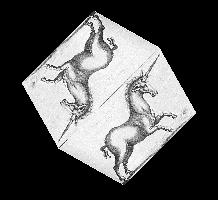
\includegraphics[width=0.6602in,height=0.6602in]{ub-img/ub-img24.jpg}
\end{center}
\\\hline
Sphere

~

~

Cylinder &
The y texture coordinate ranges linearly from 0.0 to 1.0. On spheres
this is from\newline
z= -radius to z=radius; on cylinders, from\newline
z = 0 to z = height. \ The x texture coordinate ranges from 0.0 at the
positive y-axis to 0.25 at the positive x-axis, to 0.5 at the
negative\newline
y-axis to 0.75 at the negative x-axis back to 1.0 at the positive
y-axis.  &
None &


\begin{center}
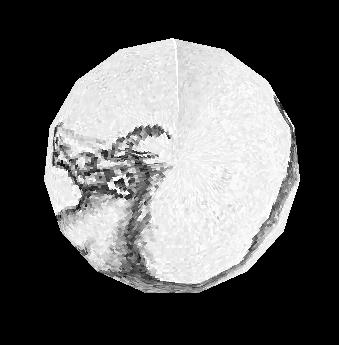
\includegraphics[width=0.6602in,height=0.6602in]{ub-img/ub-img25.jpg}
\end{center}
\begin{center}
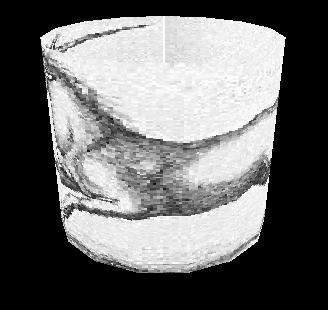
\includegraphics[width=0.6602in,height=0.6602in]{ub-img/ub-img26.jpg}
\end{center}
\\\hline
Filled Polygon

~

Line

~

~

Polygon

~

Segment

~
 &
The x and y texture coordinates are given by
p\textsubscript{1}x\textsubscript{0}+p\textsubscript{2}y\textsubscript{0}+p\textsubscript{3}z\textsubscript{0}+p\textsubscript{4}w\textsubscript{0}
 &
A texture coordinate is assigned to a vertex.  &


\begin{center}
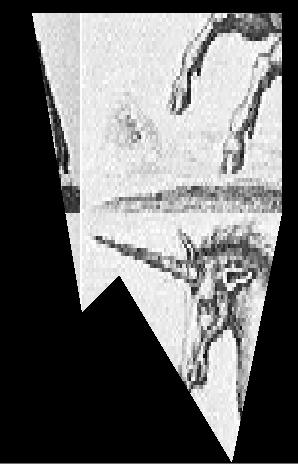
\includegraphics[width=0.6602in,height=0.6602in]{ub-img/ub-img27.jpg}
\end{center}
\begin{center}

\includegraphics[width=0.6602in,height=0.6602in]{ub-img/ub-img28.jpg}
\end{center}
\begin{center}
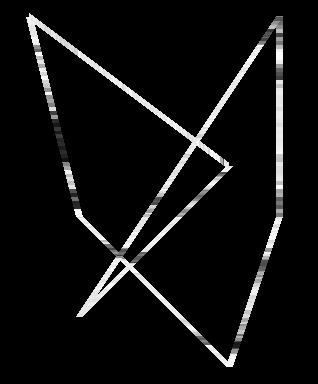
\includegraphics[width=0.6602in,height=0.6602in]{ub-img/ub-img29.jpg}
\end{center}
\begin{center}
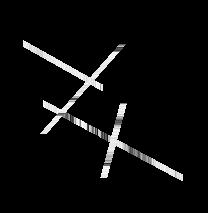
\includegraphics[width=0.6602in,height=0.6602in]{ub-img/ub-img30.jpg}
\end{center}
\\\hline
Torus &
The x and y texture coordinates are given by
p\textsubscript{1}x\textsubscript{0}+p\textsubscript{2}y\textsubscript{0}+p\textsubscript{3}z\textsubscript{0}+p\textsubscript{4}w\textsubscript{0}
&
None &
\begin{center}
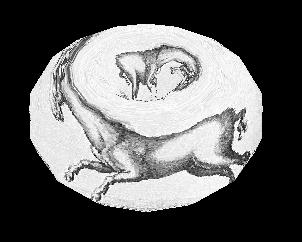
\includegraphics[width=0.6693in,height=0.698in]{ub-img/ub-img31.jpg}
\end{center}
\\\hline
\end{supertabular}
\end{center}

\subsubsection{Examples}

The following section provides examples and a further description of the
Unicon 3D graphics facilities. 

\paragraph{Changing Context Attributes}
The user can change attributes throughout a program, and multiple
attributes can be changed with one call to WAttrib(). This is
illustrated in the following line of code, which changes the eye
position to (0.0, 0.0, 5.0) and the eye direction to look at the
positive z-axis. An assignment to eyepos, eyedir, eyeup\texttt{ }or eye
redraws the screen; a given call to WAttrib() will only redraw the
scene once.

\iconcode{
\>   WAttrib({\textquotedbl}eyepos=0.0,0.0,5.0{\textquotedbl},{\textquotedbl}eyedir=0.0,0.0,1.0{\textquotedbl})}

The values of the attributes can also be read by using the function
WAttrib(). The \ current eye position could be stored in variable ep by
the call:

\iconcode{
\>   ep := WAttrib({\textquotedbl}eyepos{\textquotedbl})}

\paragraph{Drawing Primitives}
The following is an example on how to use some of the functions to draw
primitives. 

\iconcode{
\>   Fg(w, {\textquotedbl}ambient yellow{\textquotedbl}) \\
\>   DrawDisk(w, 0.4, -0.5, -4.0, 0.0, 1.0, 0.0, 0.0, 1.0,
		 0.5, -5.0, 0.5, 1.0) \\
\>   Fg(w, {\textquotedbl}diffuse white{\textquotedbl}) \\
\>   DrawDisk(w, 0.4, -0.5, -4.0, 0.0, 1.0, 0.0, 
		225.0,1.0, 0.5, -5.0, 0.5,1.0,0.0,125.0) \\
\>   Fg(w, {\textquotedbl}ambient pink{\textquotedbl}) \\
\>   DrawCylinder(w, \ 0.0, 1.0, -5.0, 1.0, 0.5, 0.3) \\
\>   Fg(w, {\textquotedbl}specular navy{\textquotedbl}) \\
\>   DrawDisk(w, -0.5, -0.5, -2.0, 0.5, 0.3) \\
\>   Fg(w, {\textquotedbl}emission green{\textquotedbl}) \\
\>   DrawSphere(w, 0.5, 1.0, -3.0, 0.5) \\
\>   WAttrib(w, {\textquotedbl}light0=on, diffuse white{\textquotedbl})
}

% \clearpage

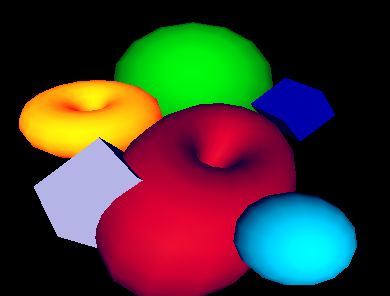
\includegraphics[width=2.8071in,height=2.1335in]{ub-img/ub-img32.png} 

{\sffamily\bfseries Figure 7-2:}
{\sffamily 3D Drawing Primitives Made From Various Materials}

\bigskip

The function Fg() specifies the material properties of an object. These
material properties affect the color and appearance of the primitives.
\ After a call to Fg(), all objects will be drawn with the material
properties until the material property is changed with another call to
Fg().\texttt{ }In this example, a cube with a diffuse green material is
drawn with sides of length 0.7. Then a sphere with a diffuse purple and
ambient blue material is drawn with radius 0.5 and center (0.4, -0.5,
-4.0). Next a diffuse yellow and ambient grey torus with center (-1.0,
0.4, -4.0), an inner radius of 0.4, and an outer radius of 0.5 is
drawn. Finally a filled polygon with a diffuse red material property
and three vertices,\texttt{ }(0.25, -0.25, -1.0), (1.0, 0.25, -4.0) and
(1.3, -0.4, -3.0) is drawn. 

\paragraph{Lighting and Materials}
There are a maximum of eight lights that can be used in each scene. The
lights are control by the context attributes light0 through light7.
Each light has five properties that can be changed throughout the
program, ambient, diffuse, specular, position, and on/off. \ The
properties of a light can be changed by using WAttrib() and one of
light0 through light7. \ To turn on or off a light, one can assign on
or off to the light, followed by a comma and a lighting value. A
lighting value is a string which contains one or more semi-colon
separated lighting properties. A lighting property is of the form
\newline
 \ \ [diffuse{\textbar}ambient{\textbar}specular] \textit{color
name}\newline
If one does not want to turn on or off a light, a lighting value is
specified. The following call turns light1 on and gives it diffuse
yellow and ambient gold lighting properties. 

\ \ \ WAttrib(w, {\textquotedbl}light1=on, diffuse yellow; ambient
gold{\textquotedbl})

The following expression sets \textsf{light0} to the default values for
the lighting properties.

\iconcode{
\>   WAttrib(w, {\textquotedbl}light0=diffuse white; ambient black; \_ \\
\>   \ \ \ \ \ \ \ \ \ \ \ \ \ \ \ \ \ \ \ specular white; position
0.0, 1.0, 0.0{\textquotedbl})}

The next example shows the difference between the different types of
lighting that can be used in a scene. Each window is the same scene
rendered using different lighting. The upper right scene has an ambient
blue-green light. The upper left scene was drawn using a diffuse
blue-green light. The lower right scene uses only a specular blue-green
light. The scene in the lower left uses all three types of lighting.

{\centering 
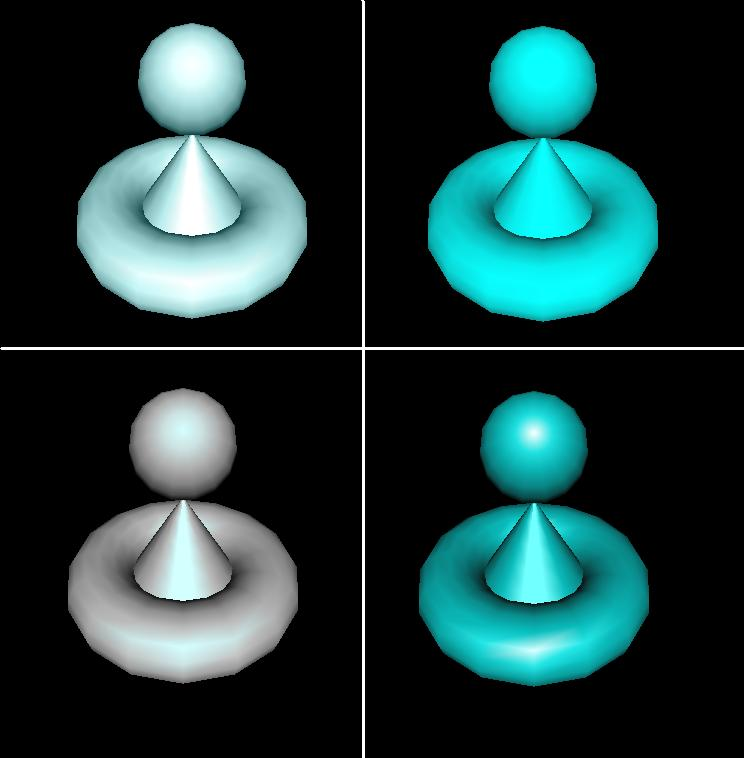
\includegraphics[width=2.1957in,height=2.2346in]{ub-img/ub-img33.jpg}
\par}

{\sffamily\bfseries Figure 7-3:}
{\sffamily Different Types of Lighting}

\bigskip

\iconcode{
\>   w :=
open({\textquotedbl}ambient.icn{\textquotedbl},{\textquotedbl}gl{\textquotedbl},
{\textquotedbl}bg=black{\textquotedbl},
{\textquotedbl}size=400,400{\textquotedbl}) \\
\>   WAttrib(w,{\textquotedbl}light0=on, ambient
blue-green{\textquotedbl},{\textquotedbl}fg=specular
white{\textquotedbl}) \\
\>   DrawCylinder(w, 0.0, -0.2, -3.5, 0.75, 0.5, 0.0) \\
\>   DrawTorus(w,0.0, -0.2, -3.5, 0.3, 0.7) \\
\>   DrawSphere(w,0.0, 0.59, -2.2, 0.3) \\
\ \\
\>   x :=
open({\textquotedbl}diffuse.icn{\textquotedbl},{\textquotedbl}gl{\textquotedbl},
{\textquotedbl}bg=black{\textquotedbl},
{\textquotedbl}size=400,400{\textquotedbl}) \\
\>   WAttrib(x,{\textquotedbl}light0=on, diffuse
blue-green{\textquotedbl},{\textquotedbl}fg=specular
white{\textquotedbl}) \\
\>   DrawCylinder(x, 0.0, -0.2, -3.5, 0.75, 0.5, 0.0) \\
\>   DrawTorus(x,0.0, -0.2, -3.5, 0.3, 0.7) \\
\>   DrawSphere(x, 0.0, 0.59, -2.2, 0.3) \\
\ \\
\>   y :=
open({\textquotedbl}specular.icn{\textquotedbl},{\textquotedbl}gl{\textquotedbl},
{\textquotedbl}bg=black{\textquotedbl},
{\textquotedbl}size=400,400{\textquotedbl}) \\
\>   WAttrib(y,{\textquotedbl}light0=on,specular
blue-green{\textquotedbl},{\textquotedbl}fg=specular
white{\textquotedbl}) \\
\>   DrawCylinder(y, 0.0, -0.2, -3.5, 0.75, 0.5, 0.0) \\
\>   DrawTorus(y, 0.0, -0.2, -3.5, 0.3, 0.7) \\
\>   DrawSphere(y, 0.0, 0.59, -2.2, 0.3) \\
\ \\
\>   z :=
open({\textquotedbl}all.icn{\textquotedbl},{\textquotedbl}gl{\textquotedbl},
{\textquotedbl}bg=black{\textquotedbl},
{\textquotedbl}size=400,400{\textquotedbl}) \\
\>   WAttrib(z, {\textquotedbl}light0=on, diffuse blue-green; \_ \\
\>   \ specular blue-green; ambient
blue-green{\textquotedbl},{\textquotedbl}fg=specular
white{\textquotedbl}) \\
\>   DrawCylinder(z, 0.0, -0.2, -3.5, 0.75, 0.5, 0.0) \\
\>   DrawTorus(z, 0.0, -0.2, -3.5, 0.3, 0.7) \\
\>   DrawSphere(z, 0.0, 0.59, -2.2, 0.3)
}

Materials can be changed using Fg() or WAttrib() with the context
attribute fg. A material value is a string containing one or more
semi-colon separated material properties. Material properties are of
the form\newline
\ \ [ diffuse {\textbar} ambient {\textbar} specular {\textbar} emission
] \textit{color name} \newline
or \newline
\ \ {\textquotedbl}shininess n{\textquotedbl}, where n is some integer
in the range 0 {\textless}= n
{\textless}= 128.

The default material property type is diffuse, so the call
Fg({\textquotedbl}red{\textquotedbl}) is equivalent to
Fg({\textquotedbl}diffuse red{\textquotedbl}). For shininess, a value
of 0 spreads specular light broadly across an object and a value of 128
focuses specular light at a single point. The following line of code
changes the current material property to diffuse green and ambient
orange. 

\iconcode{
\ \ \ WAttrib(w, {\textquotedbl}fg=diffuse green; ambient
orange{\textquotedbl})
}

\noindent The default values of the material properties are given in the
following example. 

\iconcode{
   Fg(w, \textrm{{\textquotedbl}}diffuse light grey; ambient grey;
specular black; emission black; \_ \\
\>\> shininess 50\textrm{{\textquotedbl}})}

\noindent Figure 7-4 \ shows the effects of emission color on an object. 

\bigskip

{\centering 
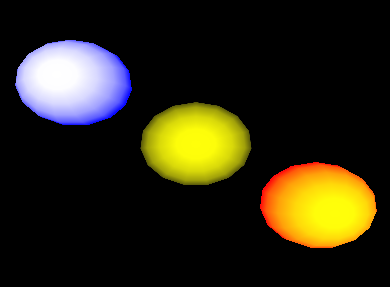
\includegraphics[width=2.5583in,height=1.8835in]{ub-img/ub-img34.png}
\par}

{\sffamily\bfseries Figure 7-4:}
{\sffamily Mixing Emission and Diffuse Material Properties}

\bigskip

\iconcode{
\>   Fg(w, {\textquotedbl}emission blue; diffuse yellow{\textquotedbl}) \\
\>   DrawSphere(w, -1.5, 1.0, -5.0, 0.7) \\
\>   Fg(w, {\textquotedbl}emission black{\textquotedbl}) \\
\>   DrawSphere(w, 0.0, 0.0, -5.0, 0.7) \\
\>   Fg(w, {\textquotedbl}emission red{\textquotedbl}) \\
\>   DrawSphere(w, 1.5, -1.0, -5.0, 0.7)
}

In the above example, three yellow spheres are drawn. If an emission
color of blue is applied to the sphere, the sphere appears white with a
blue ring. If the emission color is red, the sphere remains yellow, but
now has an orange-red ring. The middle sphere shows the effect of
having no emission color. In order to obtain the diffuse yellow sphere
in the center, the emission color was changed to black, without
changing the diffuse property.

\paragraph{Textures}
This section contains several examples of the use of textures in a
scene. There are several ways to specify the texture image: a file, an
image string, or another Unicon window. The following example shows how
to use a file as a texture. A .gif image of a map of the word is used
to texture a torus. The texture coordinates are the default
coordinates.

\clearpage

{\centering 
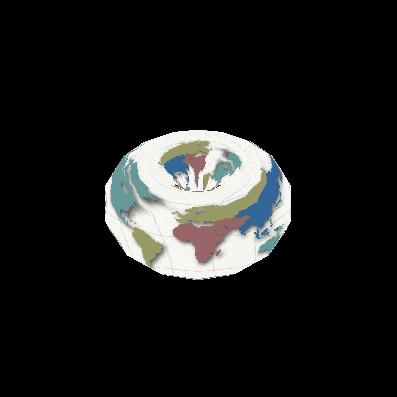
\includegraphics[width=2.0583in,height=2.0583in]{ub-img/ub-img35.jpg}
\par}

{\sffamily\bfseries Figure 7-5:}
{\sffamily A Texture from a GIF Image is Mapped onto a Torus}

\bigskip

\iconcode{
\>   WAttrib(w, {\textquotedbl}texmode=on{\textquotedbl},
{\textquotedbl}texture=map.gif{\textquotedbl}) \\
\>   DrawTorus(w, 0.0, 0.0, -3.0, 0.3, 0.4)
}

Instead of using \textsf{WAttrib(w,
{\textquotedbl}texture=map.gif{\textquotedbl})}\texttt{ }to specify the
.gif file, a call to \textsf{Texture(w,
{\textquotedbl}map.gif{\textquotedbl})} could be used to obtain the
same result.

The next example illustrates the use of an image string to specify a
texture image. The string used for this example is taken from Graphics
Programming in Icon [Griswold98] page 156. This string is used as a
texture on a cube using the default texture coordinates. 

\bigskip

{\centering 
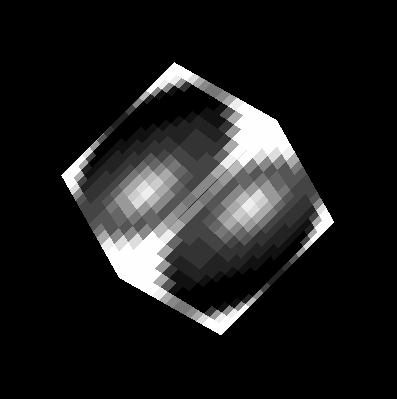
\includegraphics[width=2.0508in,height=2.0571in]{ub-img/ub-img36.jpg}
\par}

{\sffamily\bfseries Figure 7-6:}
{\sffamily A Texture Supplied via an Image String}

\bigskip

\iconcode{
\ \ \ WAttrib(w, {\textquotedbl}texmode=on{\textquotedbl}) \\
\>   sphere:= {\textquotedbl}16,g16, FFFFB98788AEFFFF{\textquotedbl}
{\textbar}{\textbar} \\
\>   \ \ {\textquotedbl}FFD865554446AFFF FD856886544339FF
E8579BA9643323AF{\textquotedbl}{\textbar}{\textbar} \\
\>   \ \ {\textquotedbl}A569DECA7433215E 7569CDB86433211A
5579AA9643222108{\textquotedbl}{\textbar}{\textbar} \\
\>   \ \ {\textquotedbl}4456776533221007 4444443332210007
4333333222100008{\textquotedbl}{\textbar}{\textbar} \\
\>   \ \ {\textquotedbl}533322221100000A 822222111000003D
D41111100000019F{\textquotedbl}{\textbar}{\textbar} \\
\>   \ \ {\textquotedbl}FA200000000018EF FFA4000000028EFF
FFFD9532248BFFFF{\textquotedbl} \\
\>   Texture(w, sphere) \\
\>   DrawCube(w, 0.0, 0.0, -3.0, 1.2)
}

The next example shows the use of another Unicon window as a texture. A
simple scene of a lamp is drawn on the first window in
{\textquotedbl}\textsf{gl{\textquotedbl}} mode. This window is then
captured and used as a texture on a cylinder. The same method can be
used to embed 2D window contents in 3D scenes. Note that in the
following code the first window is opened with size 256 x 256. Texture
images must have height and width that are powers of 2, or the system
must rescale them. The default coordinates for cylinders are used.

{\centering\color{green}
 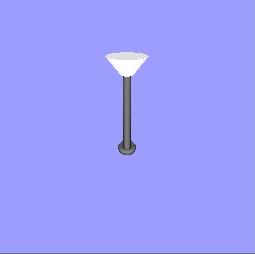
\includegraphics[width=1.4492in,height=1.4335in]{ub-img/ub-img37.jpg}
\texttt{ \ \ }

\includegraphics[width=1.939in,height=1.952in]{ub-img/ub-img38.jpg}
\texttt{ \ \ }
\par}

{\sffamily\bfseries Figure 7-7:}
{\sffamily A Texture Obtained from Another Window{\textquotesingle}s Contents}

\bigskip

\iconcode{
\>   w :=
open({\textquotedbl}win1{\textquotedbl},{\textquotedbl}gl{\textquotedbl},{\textquotedbl}bg=light
blue{\textquotedbl},{\textquotedbl}size=256,256{\textquotedbl}) \\
\>   Fg(w, {\textquotedbl}emission pale grey{\textquotedbl}) \\
\>   PushMatrix(w) \\
\>   Rotate(w, -5.0, 1.0, 0.0, 0.0) \\
\>   DrawCylinder(w, 0.0, 0.575, -2.0, 0.15, 0.05, 0.17) \\
\>   PopMatrix(w) \  \\
\>   Fg(w, {\textquotedbl}diffuse grey; emission black{\textquotedbl}) \\
\>   PushMatrix(w) \\
\>   Rotate(w, -5.0, 1.0, 0.0, 0.0) \\
\>   DrawCylinder(w, 0.0, 0.0, -2.5, 0.7, 0.035, 0.035) \\
\>   PopMatrix(w) \ \ \ \ \ \ \ \ \ \ \ \ \ \  \\
\>   DrawTorus(w, 0.0, -0.22, -2.5, 0.03, 0.06) \\
\>   DrawTorus(w, 0.0, 0.6, -2.5, 0.05, 0.03) \\
\ \\
\>   w2 :=
open({\textquotedbl}win2.icn{\textquotedbl},{\textquotedbl}gl{\textquotedbl},{\textquotedbl}bg=black{\textquotedbl},{\textquotedbl}size=400,400{\textquotedbl}) \\
\>   WAttrib(w2, {\textquotedbl}texmode=on{\textquotedbl}) \\
\>   Texture(w2, w)  \\
\>   Fg(w2, {\textquotedbl}diffuse purple; ambient blue{\textquotedbl}) \\
\  \\
\>   DrawCylinder(w2, 0.0, 0.0, -3.5, 1.2, 0.7, \ 0.7)
}

The next two examples illustrate the use of the default texture
coordinates versus texture coordinates specified by the programmer. In
both examples, a bi-level image is used as the texture image. The
format for such a string is described in section 2.7. This image is
taken from Graphics Programming in Icon page 159. The first example
uses the default texture coordinates for a filled polygon, which in
this case is just a square with sides of length one. In this case the
default texture coordinates are as follows. The coordinate (0.0,
0.0)\textsf{ }of the texture image is mapped to the vertex\texttt{
}(0.0, 0.0, -2.0) of the square, (0.0, 1.0)\textsf{ }is mapped to (0.0,
1.0, -2.0)\textsf{, }(1.0, 1.0)\texttt{ }is mapped to (1.0, 1.0, -2.0),
and (1.0, 0.0)\textsf{ }is mapped to (1.0, 0.0, -2.0).

{\centering 
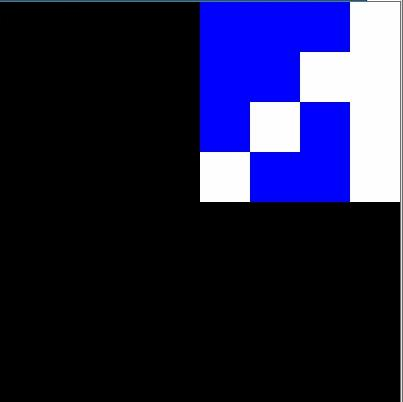
\includegraphics[width=1.8335in,height=1.8335in]{ub-img/ub-img39.jpg}
\par}

{\sffamily\bfseries Figure 7-8:}
{\sffamily Default Texture Coordinates}

\bigskip

\iconcode{
\>   WAttrib(w,{\textquotedbl}fg=white{\textquotedbl},{\textquotedbl}bg=blue{\textquotedbl},{\textquotedbl}texmode=on{\textquotedbl},{\textquotedbl}texture=4,\#8CA9{\textquotedbl}) \\
\>   Fg(w, {\textquotedbl}diffuse purple; ambient blue{\textquotedbl}) \\
\>   FillPolygon(w, 0.0, 0.0, -2.0, 0.0, 1.0, -2.0, \\
\>   \ \ \ \ \ \ \ \ \ \ \ \ \ \ \ 1.0, 1.0, -2.0, 1.0, 0.0, -2.0)
}

This example uses the same texture image and the same object to be
textured, but instead uses the texture coordinates (0.0, 1.0), (1.0,
1.0), (1.0, 1.0), and (1.0, 0.0). So the coordinate (0.0, 1.0) of the
texture image is mapped to the vertex (0.0, 0.0, -2.0) of the square,
(1.0, 1.0) is mapped to (0.0, 1.0, -2.0),(1.0, 1.0) is mapped to (1.0,
1.0, -2.0), and (1.0, 0.0) is mapped to (1.0, 0.0, -2.0).

\bigskip

{\centering 
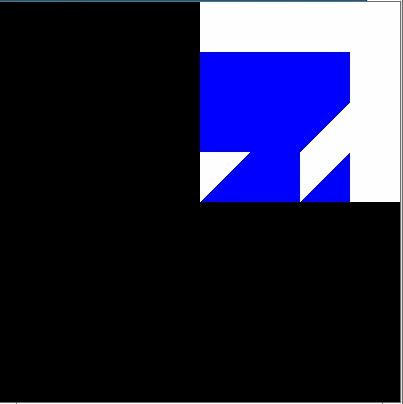
\includegraphics[width=2.0307in,height=2.0311in]{ub-img/ub-img40.jpg}
\par}

{\sffamily\bfseries Figure 7-9:}
{\sffamily Custom Texture Coordinates}

\bigskip

\iconcode{
\>   Wattrib(w,{\textquotedbl}fg=white{\textquotedbl},{\textquotedbl}bg=blue{\textquotedbl},{\textquotedbl}texmode=on{\textquotedbl},{\textquotedblright}texture=4,\#8CA9{\textquotedblright}, \\
\>   \ \ \ \ \ \ \ \ \ \ {\textquotedbl}texcoord=0.0, 1.0, 1.0, 1.0,
1.0, 1.0, 1.0, 0.0{\textquotedbl}) \\
\>   FillPolygon(w, 0.0, 0.0, -2.0, 0.0, 1.0, -2.0, \\
\>   \ \ \ \ \ \ \ \ \ \ \ \ \ \ \ 1.0, 1.0, -2.0, 1.0, 0.0, -2.0)
}

Instead of using WAttrib() with the attribute texcoord, the function
Texcoord() could be used. So the line 

\iconcode{
\>   WAttrib(w,{\textquotedbl}texcoord=0.0, 1.0, 1.0, 1.0, 1.0,
1.0,1.0, 0.0{\textquotedbl})}

could be replaced by 

\iconcode{
\>   Texcoord(w, 0.0, 1.0, 1.0, 1.0, 1.0, 1.0,1.0, 0.0)}

\paragraph[A Larger Textures Example]{A Larger Textures Example}
The following is a more complicated example that uses many features of
the Unicon 3D graphics facilities described in the previous sections.
This example also illustrates the effect that adding texture to a scene
can have. The scene on the left is a scene drawn without any texturing.
The scene on the right contains texturing. The scene on the right is a
much more realistic scene than the one on the left. 

All textures used in the textured scene, except for the unicorn, where
captured using a digital camera. These images were then converted into
.gif files and scaled to width and height of 2\textsuperscript{n}.
Directly using an image file is one feature of the Unicon 3D graphics
facilities that makes adding textures simpler than using OpenGL. 

\bigskip

{\color{green}
 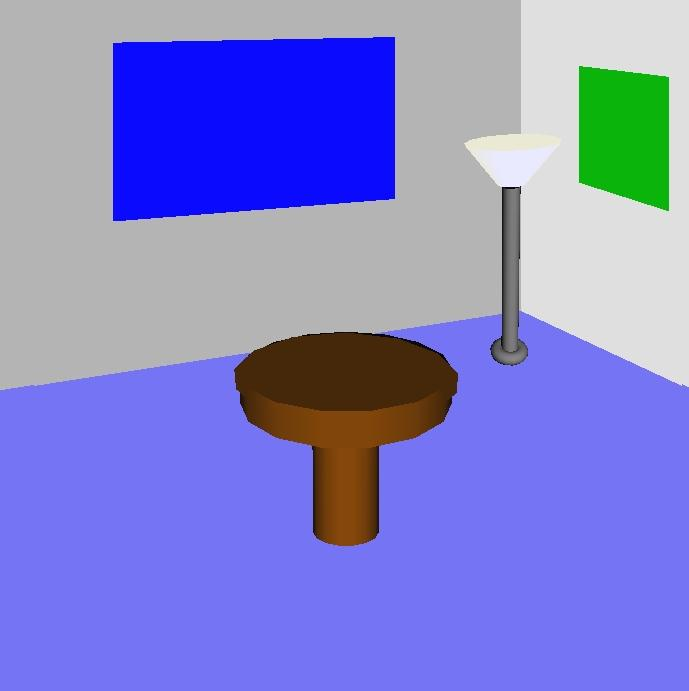
\includegraphics[width=2.6543in,height=2.6693in]{ub-img/ub-img41.jpg}
\textbf{ \ \ \ \ \ \ \ \ \ \ \ \ \ }
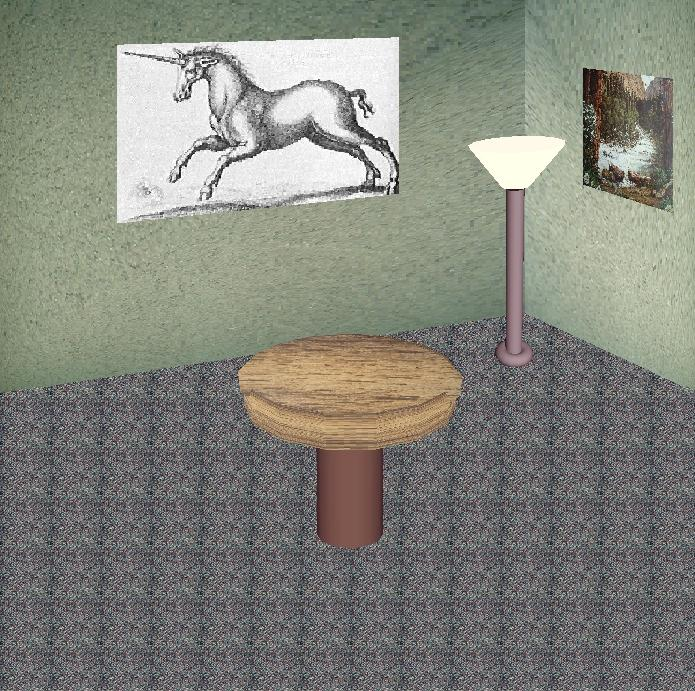
\includegraphics[width=2.6846in,height=2.6693in]{ub-img/ub-img42.jpg} }

{\sffamily\bfseries Figure 7-10:}
{\sffamily\bfseries Untextured and Textured Versions of the Same Scene}

\bigskip

\iconcode{
procedure main() \\
\>   \&window
:=open({\textquotedbl}textured.icn{\textquotedbl},{\textquotedbl}gl{\textquotedbl},{\textquotedbl}bg=black{\textquotedbl},{\textquotedbl}size=700,700{\textquotedbl}) \\
\ \\
\>   \# Draw the floor of the room \\
\>   WAttrib({\textquotedbl}texmode=on{\textquotedbl},
{\textquotedbl}texture=carpet.gif{\textquotedbl}) \\
\>   FillPolygon(-7.0, -0.9, -14.0, -7.0, -7.0, -14.0, \\
\>\>\> 7.0, -7.0,
-14.0, 7.0, -0.9, -14.0, 3.5, 0.8, -14.0) \\
\ \\
\>   \# Draw the right wall \\
\>   Wattrib({\textquotedbl}texture=wall1.gif{\textquotedbl},
{\textquotedbl}texcoord=0.0, 1.0, 0.0, 0.0, 1.0, 0.0, 1.0,
1.0{\textquotedbl}) \\
\>   FillPolygon(2.0, 4.0, -8.0, 8.3, 8.0, -16.0, 8.3, -1.2, -16.0,
2.0, 0.4, -8.0) \\
\ \\
\>   \# Draw the left wall \\
\>   WAttrib({\textquotedbl}texture=wall2.gif{\textquotedbl}) \\
\>   FillPolygon(2.0, 4.0 ,-8.0, -9.0, 8.0, -16.0, -9.0,-1.2,-16.0,
2.0, 0.4, -8.0) \\
\ \\
\>   \# Draw a picture \\
\>   Wattrib({\textquotedbl}texture=poster.gif{\textquotedbl},
{\textquotedbl}texcoord=0.0, 1.0, 0.0, 0.0, 1.0, 0.0, 1.0,
1.0{\textquotedbl}) \\
\>   FillPolygon(1.0, 1.2, -3.0, 1.0, 0.7, -3.0, 1.2, 0.5, -2.6, 1.2,
1.0, -2.6) \\
\>   \# Draw another picture \\
\>   Wattrib({\textquotedbl}texture=unicorn.gif{\textquotedbl},
{\textquotedbl}texcoord=1.0, 0.0, 0.0, 0.0, 0.0, 1.0, 1.0,
1.0{\textquotedbl}) \\
\>   FillPolygon(0.8, 2.0, -9.0, -3.0, 1.6, -9.0, 3.0, 3.9,-9.0, 0.8,
4.0, -9.0)
\ \\
\>   \# Draw the lamp \\
\>   WAttrib({\textquotedbl}texmode=off{\textquotedbl}) \\
\>   PushMatrix() \\
\>   Translate(0.7, 0.20, -0.5) \\
\>   Fg({\textquotedbl}emission pale weak yellow{\textquotedbl}) \\
\>   PushMatrix() \\
\>   Rotate(-5.0, 1.0, 0.0, 0.0) \\
\>   Rotate( 5.0, 0.0, 0.0, 1.0) \\
\>   DrawCylinder(-0.05, 0.570, -2.0, 0.15, 0.05, 0.17) \\
\>   PopMatrix() \\
\>   Fg({\textquotedbl}diffuse grey; emission black{\textquotedbl}) \\
\>   PushMatrix() \\
\>   Rotate(-5.0, 1.0, 0.0, 0.0) \\
\>   Rotate( 6.0, 0.0, 0.0, 1.0) \\
\>   DrawCylinder(0.0, 0.0, -2.5, 0.7, 0.035, 0.035) \\
\>   PopMatrix() \\
\>   PushMatrix() \\
\>   Rotate(6.0, 0.0, 0.0, 1.0) \\
\>   DrawTorus(-0.02, -0.22, -2.5, 0.03, 0.05) \\
\>   PopMatrix() \  \\
\>   PopMatrix()
\ \\
\>   \# Draw the table  \\
\>   WAttrib({\textquotedbl}texcoord=auto{\textquotedbl},
{\textquotedbl}texmode=on{\textquotedbl},
{\textquotedbl}texture=table.gif{\textquotedbl}) \\
\ \\
\>   PushMatrix() \\
\>   Rotate(-10.0, 1.0, 0.0,0.0) \\
\>   DrawCylinder(0.0, 0.2, -2.0, 0.1, 0.3, 0.3) \\
\>   PopMatrix() \\
\ \\
\>   PushMatrix() \\
\>   Translate(0.0, -0.09, -1.8) \\
\>   Rotate(65.0, 1.0, 0.0, 0.0) \\
\>   DrawDisk(0.0, 0.0, 0.0, 0.0, 0.29)  \\
\>   PopMatrix() \\
\ \\
\>   WAttrib({\textquotedbl}texmode=off{\textquotedbl},
{\textquotedbl}fg=diffuse weak brown{\textquotedbl}) \\
\>   PushMatrix() \\
\>   Rotate(-20.0, 1.0, 0.0,0.0) \\
\>   DrawCylinder(0.0, 0.2, -2.2, 0.3, 0.1, 0.1) \\
\>   PopMatrix() \\
\>   while (e := Event()) \~{}== {\textquotedbl}q{\textquotedbl} do \{ \\
\>   \ \ \ write(image(e), {\textquotedbl}: {\textquotedbl}, \&x,
{\textquotedbl},{\textquotedbl}, \&y) \\
\>   \ \ \ \} \\
end
}

In order to apply textures to the scene, texturing must first be turned
on. Next, the texture to be applied is specified. The floor of the
scene is drawn using a filled polygon. The default texture coordinates
are used to apply the carpet texture to the floor of the room. The
tiled appearance on the floor of the room is caused by the use of the
default texture coordinates. \ This can be avoided by using user
defined texture coordinates. This is what is done for the textures that
are applied to the two walls of the room and the pictures. 

The lamp does not have any texturing applied to it, so it is necessary
to turn off texturing before drawing the lamp. Also for the lamp to be
centered properly in the room, transformations are used. Notice the use
of matrices to isolate the transformations of the lamp. Finally to draw
the table with a textured top and an untextured base, two cylinders and
a disk are used. Texturing is applied to a cylinder and the disk.
Notice the call 

\ \ \ WAttrib(w, {\textquotedbl}texcoord=auto{\textquotedbl})

This resets the texture coordinates to the defaults. Finally, texturing
is turned off to draw the base of the table.

\subsubsection{Animation}

Graphics animation is performance sensitive, and Unicon is slower than
systems programming languages such as C and C++. Nevertheless, it is
possible to write 3D animations in Unicon with acceptable frame rates.

3D animations redraw the entire scene each time any object has moved, or
the user has changed point of view. An application can call EraseArea()
followed by the appropriate graphics primitives to redraw a scene, but
the results often appear to flicker. It is better to let
Unicon{\textquotesingle}s runtime system do the redrawing. \ Unicon
maintains a \textit{display list} of graphics operations to execute
whenever the screen must be redrawn; these operations are effectively
everything since the last EraseArea(). The display list for a window
can be obtained by calling WindowContents(). The elements of the list
are Unicon records and lists containing the string names and parameters
of graphics primitives. \ For example, a call to DrawSphere(w,x,y,z,r)
returns (and adds to the display list) a record
gl\_sphere({\textquotedbl}DrawSphere{\textquotedbl},x,y,z,r). Instead
of redrawing the entire scene in order to move an object, you can
modify its display list record and call Refresh(). The following code
fragment illustrates animation by causing a ball to slide up and down.
In order to \textit{bounce}, the program would need to incorporate
physics. 

\iconcode{
sphere := DrawSphere(w, x, y, z, r) \\
increment := 0.2 \\
every i := 1 to 100 do \\
\>   every j := 1 to 100 do \{ \\
\>   \ \ \ sphere.y +:= increment \\
\>   \ \ \ Refresh(w) \\
\>   \ \ \ \}
}

This technique gives animation rates of 100-200 frames per second on
current midrange PC hardware. Unicon supports smooth animation for a
number of objects which varies widely depending on the underlying
graphics hardware and software.

\subsubsection{Selective Rendering and Object Selection}

Many 3D applications model scenes with far more objects than are needed
at any particular instant. For example, a virtual building might have
many rooms on multiple floors, but only a small fraction is visible
from any particular location. The 3D facilities remove objects that are
not visible, but doing so becomes too slow for large numbers of
objects. An application with a large scene will generally have to
perform at least approximate visibility calculations to achieve smooth
animation. Such visibility calculations can be performed for each
frame, and if the visible objects change, the scene can be re-rendered
by rebuilding the display list from scratch. At this point
Unicon{\textquotesingle}s speed can be an issue, as discussed in the
previous section.

The function \textsf{WSection()} comes to the rescue. It plays two vital
roles. First, it allows portions of the display list to be skipped
during rendering, without having to rebuild the display list. Second,
it forms the basis for specifying portions of the display list that the
user may select (click on) when interacting with the scene. In both
cases, calls to \textsf{WSection()} come in pairs, first a call
\textsf{WSection(s)} identifies a portion of the display list of
interest, then the sequence of 3D calls to render some object or
portion of the scene, then a call to \textsf{WSection()} defines the
end of that section. Parameter \textsf{s} must be a unique string name
or identifier for the section.

The call to create a new section returns a record that contains a field
named skip. Setting skip to a non-null value causes the section to be
omitted whenever the scene is redrawn.

Using \textsf{WSection()} for 3D user input is similar. A program calls
\textsf{WAttrib({\textquotedblleft}pick=on{\textquotedblright})} to
turn on 3D selection, after which keyword \textsf{\&pick} generates the
identifying names for all objects intersected by the ray from the
camera through the (x,y) screen location where the mouse was located on
the last call to \textsf{Event()}.

\section*{Summary}

Graphics are ubiquitous in modern applications. Unicon provides 2D and
3D graphics capabilities that are easy to use, portable building blocks
for many programs. \ The 2D facilities are mature; the 3D interface is
new and will evolve. Many elements of the 2D graphics system are used
in the 3D graphics interface. Further integration of the 2D and 3D
graphics systems is likely in the future.


\bigskip

\clearpage
\bigskip

\clearpage
\bigskip
